% \loop\iftrue%
\errmessage{This article is copyrighted by ___ and should not be TeXed}%
\repeat%

\documentclass{ifacconf}  % Comment this line out
\usepackage{natbib}        % required for bibliography

% \documentclass[a4paper, 10 pt, conference]{ieeeconf}  % Comment this line out
% \IEEEoverridecommandlockouts%
\pdfminorversion=4%

\usepackage{graphicx}      % include this line if your document contains figures
\usepackage{grffile}       % filenames
\usepackage{booktabs}       % filenames
\usepackage{xparse}
% \usepackage{hyperref}
\usepackage{tikz}
\usetikzlibrary {graphs}

\usepackage{tikzscale}
\usepackage{bm}
\usepackage{ifthen}
\usepackage[ruled,noend,algo2e]{algorithm2e}
\SetKwRepeat{Do}{do}{while}

\usepackage[justification=centering]{caption}
\usepackage{subcaption}
% \usepackage{pdfcomment}


% \newcommand{\symbl}[3]{\newglossaryentry{#1}{name ={#2},	description ={#3}}
%   \expandafter\newcommand\csname #1\endcsname{\gls{#1}}
% }




\usepackage{color}
\newcommand{\no}[1]{}

\def\maybeonecolumn{}

\makeatletter
\def\comments{
  \usepackage{geometry}
  \newgeometry{
    textwidth=8cm,
    hoffset=-1.5in,
    bottom=0.41in,
    vscale=.5,
    % height=.2\textheight,
    top=0.41in,
    footskip=1cm,
  }
\@TwoColumnfalse
\@twocolumnfalse
}
\makeatother

% \usepackage{stfloats}

% \usepackage[showframe]{geometry}
% \usepackage{geometry}
% \geometry{
%   top=19.1mm,
%   bottom=36.7mm,
%   left=19.1mm,
%   right=13.1mm,
% }



\newif\ifdebug%
\newcommand{\draft}{\debugtrue}
\newcommand{\final}{\debugfalse}
\newcommand{\todo}[2][FORGOT TO DO SOMETHING]{\ifdebug%
  {
    \color{red}
    #2}\else \PackageError{}{#1}{#2}#2\fi}%
\newcommand\doing[2][FORGOT TO DO SOMETHING]{\ifdebug%
  {
    \color{blue}
    #2}\else \PackageError{}{#1}{#2}#2\fi}%
\newcommand\warning[1]{\ifdebug%
  {
    \color{red}
    #1}\fi}

\makeatletter
\@ifpackageloaded{pdfcomment}
{
  \newcommand\pdfnote[1]{
    \ifdebug%
    {\pdfcomment[color=orange,opacity=0.4,subject=note]{#1}
    }\fi
  }
  \newcommand{\question}[1]{
    \ifdebug%
    {\pdfcomment[color=red,opacity=0.4,subject=Should I?]{#1}
    }\fi}
}
{
  \newcommand\pdfnote[1]{
    \ifdebug%
    {\tikz[opacity=.7]{\node[text width=2cm,align={center},color=black,fill=red,draw] {#1} }
    }\fi
  }
  \newcommand{\question}[1]{
    \ifdebug%
    {\tikz[opacity=.7]{\node[text width=2cm,align={center},rotate=2,color=black,fill=orange,draw] {#1} }
    }\fi
  }
}
\makeatother
% \newcommand\pdfnote[1]{}


%===============================================================================
\newtheorem{theorem}{theorem}[section]
\newtheorem{problem}[thm]{Problem}%[numberby]
\newtheorem{example}{Example}%[numberby]
\newtheorem{remark}{Remark}%[numberby]
\newtheorem{assumption}{Assumption}%[numberby]

\graphicspath{{../img/}}

% \makeatletter
% \hypersetup{
%   bookmarks=true,         % show bookmarks bar?
%   unicode=false,          % non-Latin characters in Acrobat’s bookmarks
%   pdftoolbar=true,        % show Acrobat’s toolbar?
%   pdfmenubar=true,        % show Acrobat’s menu?
%   pdffitwindow=false,     % window fit to page when opened
%   pdfstartview={FitH},    % fits the width of the page to the window
%   pdftitle={\@title},    % title
%   pdfauthor={\@author},     % author
%   pdfsubject={},   % subject of the document
%   pdfcreator={Rafael Accácio},   % creator of the document
%   % pdfproducer={Producer}, % producer of the document
%   pdfkeywords={keyword1, key2, key3}, % list of keywords
%   pdfnewwindow=true,                  % links in new PDF window
%   colorlinks=true,            % false: boxed links; true: colored links
%   % colorlinks=false,            % false: boxed links; true: colored links
%   linkcolor=black, % color of internal links (change box color with linkbordercolor)
%   citecolor=black,          % color of links to bibliography
%   filecolor=black,          % color of file links
%   urlcolor=black            % color of external links
% }
% \makeatother



\newcommand{\eq}[2]{\mbox{$#1=#2$}}
\newcommand{\N}{\mathbb{N}}
\newcommand{\Z}{\mathbb{Z}}
\newcommand{\Q}{\mathbb{Q}}
\newcommand{\R}{\mathbb{R}}
\newcommand{\C}{\mathbb{C}}
\newcommand{\Np}{N_{\text{p}}}
\newcommand{\T}{^{\mathrm{T}}}
\newcommand{\1}{\mathbf{1}}
\newcommand{\0}{\mathbf{0}}
\newcommand{\abs}[1]{\left\lvert#1\right\rvert}
\newcommand{\norm}[1]{\left\lVert#1\right\rVert}
\newcommand{\Varepsilon}{\mathcal{E}}
\newcommand{\diff}{\mathop{}\mathopen{}\mathrm{d}}
\newcommand{\set}[1]{\mathcal{#1}}
\newcommand{\p}{^{(p)}}
\newcommand{\pplusone}{^{(p+1)}}
\renewcommand{\vec}[1]{\boldsymbol{#1}}
\newcommand{\random}[1]{\underline{#1}}
\newcommand{\randomvec}[1]{{\underline{\vec{#1}}}}
\newcommand{\probability}[1]{\mathbb{P}(#1)}
\newcommand{\expectation}[2][]{\mathbb{E}_{#1}\left[#2\right]}
\newcommand{\indicator}[1]{\mathbb{1}_{\{#1\}}}

\newcommand{\setbuild}[2]{\{#1\mid#2\}}
\newcommand{\seq}[2][n]{\lbrace #2_{0},\ldots,\,#2_{#1} \rbrace}
\newcommand{\hadamard}[2]{#1\odot #2}
\newcommand{\kron}[2]{#1\otimes#2}
\newcommand{\vectorize}[1]{\mathrm{vec} (#1)}
\newcommand{\symmetric}{\mathbb{S}}
\newcommand{\semidefpos}{\mathbb{S}_{+}}
\newcommand{\defpos}{\mathbb{S}_{++}}
\newcommand{\elem}[2][1]{{#2}_{(#1)}}
\newcommand{\pseudoinv}[1]{{#1}^{\dagger}}
% \renewcommand{\implies}{\Rightarrow}
% \renewcommand{\iff}{\Leftrightarrow}



\usepackage{amsmath}
\usepackage{mathtools}
\usepackage{amssymb}
\DeclareMathOperator{\fix}{fix}
\DeclareMathOperator{\diag}{diag}
\DeclareMathOperator{\Proj}{Proj}
\DeclareMathOperator{\dom}{dom}
\DeclareMathOperator{\argmax}{arg\ max}
% \DeclareMathOperator{\card}{\#}
\newcommand{\card}[1]{\#(#1)}
% \DeclareMathOperator{\vector}{vec}
%

% Theorem
% \newtheorem{thm}{Theorem}[section]
% \newtheorem{lem}[thm]{Lemma}

\newcommand{\nsubsystems}{M}
\newcommand{\umax}{\vec{u}_{\mathrm{\max}}}
\newcommand{\predhorz}{N_{p}}

\NewDocumentCommand \mpcvec { s m o o o } {%
  \IfBooleanTF{#1}{
    \def\optim{^\star}
  }{
    \def\optim{}
  }
  \IfValueTF{#5}{
    \vec{#2}_{#3}\optim{}[#4|#5]
  }{
    \IfValueTF{#4}{
      \vec{#2}_{#3}\optim{}[#4]
    }
    {
    \IfValueTF{#3}{
      \vec{#2}_i\optim{}[#3]
    }
    {
      \vec{#2}_i\optim{}[k]
    }
    }
  }
}


\NewDocumentCommand \mpcval { s m o o o } {%
  \IfBooleanTF{#1}{
    \def\optim{^\star}
  }{
    \def\optim{}
  }
  \IfValueTF{#5}{
    {#2}_{#3}\optim{}[#4|#5]
  }{
    \IfValueTF{#4}{
      {#2}_{#3}\optim{}[#4]
    }
    {
    \IfValueTF{#3}{
      {#2}_i\optim{}[#3]
    }
    {
      {#2}_i\optim{}[k]
    }
    }
  }
}






\newcommand{\uikk}{\mpcvec{u}[i][k][k]}
\newcommand{\optuikk}{\mpcvec*{u}[i][k][k]}

\newcommand{\globobj}{\mpcval{J}[][k]}
\newcommand{\optglobobj}{\mpcval*{J}[][k]}

\newcommand{\obji}{\mpcval{J}[i][k]}
\newcommand{\optobji}{\mpcval*{J}[i][k]}

\newcommand{\xik}{\mpcvec{x}}
\newcommand{\fik}{\mpcvec{f}}
\newcommand{\uik}{\mpcvec{u}}
\newcommand{\uiseq}{\mpcvec{u}[i][k:k+\predhorz-1][k]}
\newcommand{\optuiseq}{\mpcvec*{u}[i][k:k+\predhorz-1][k]}

\newcommand{\useq}{\mpcvec{u}[ ][k:k+\predhorz-1][k]}
\newcommand{\optuseq}{\mpcvec*{u}[ ][k:k+\predhorz-1][k]}
\newcommand{\Uik}{\mpcvec{U}}
\newcommand{\optUik}{\mpcvec*{U}}
\newcommand{\optuncUik}{\mpcvec*{\mathring{U}}}

\newcommand{\vik}{\mpcvec{v}}
\newcommand{\wik}{\mpcvec{w}}
\newcommand{\wiseq}{\mpcvec{w}[i][k:k+\predhorz-1][k]}
\newcommand{\Wik}{\mpcvec{W}}

\newcommand{\qik}{\mpcvec{q}}
\newcommand{\qiseq}{\mpcvec{q}[i][k:k+\predhorz-1][k]}
\newcommand{\thetaik}{\mpcvec{\theta}}
\newcommand{\optthetaiseq}{\mpcvec*{\theta}[i][k:k+\predhorz-1][k]}
\newcommand{\thetaseq}{\mpcvec{\theta}[][k:k+\predhorz-1][k]}
\newcommand{\optthetaseq}{\mpcvec*{\theta}[][k:k+\predhorz-1][k]}
\newcommand{\thetai}{\vec{\theta}_i}
\newcommand{\optthetai}{\vec{\theta}_i^{\star}}

\newcommand{\dik}{\mpcvec{d}}
\newcommand{\diseq}{\mpcvec{d}[i][k:k+\predhorz-1][k]}
\newcommand{\lambdaik}{\mpcvec{\lambda}}
\newcommand{\lambdai}{\vec{\lambda}_i}
\newcommand{\lambdaicheat}{\tilde{\vec{\lambda}}_i}
\newcommand{\optlambdai}{\vec{\lambda}_i^{\star}}

\newcommand{\Tik}{\mpcval{T}}


\usepackage[acronym]{glossaries}%

\newcommand{\acrSing}[3]{\newacronym{#1}{#2}{#3}
  \expandafter\newcommand\csname #1\endcsname{\gls{#1}}}

\newcommand{\acrPl}[5]{
  \newacronym[plural=#4,firstplural=#5 (#4)]{#1}{#2}{#3}
  \expandafter\newcommand\csname #1\endcsname{\gls{#1}}
  \expandafter\newcommand\csname #4\endcsname{\glspl{#1}}
}
\newcommand{\acr}[5][4=,5=]{
  \ifthenelse{\equal{#5}{}}
  {
    \acrSing{#1}{#2}{#3}
  }
  {
    \acrPl{#1}{#2}{#3}{#4}{#5}
  }
}

\acrSing{mpc}{MPC}{Model-based Predictive Control}
\acrSing{qp}{QP}{\emph{quadratic program}}
\acrSing{dmpc}{dMPC}{distributed Model-based Predictive Control}
\acrSing{pwa}{PWA}{Piecewise Affine}
\acrSing{EM}{EM}{Expectation Maximization}
\acrSing{cps}{CPS}{cyber-physical systems}
\acrSing{fdi}{FDI}{false data injection}
\acrSing{rhs}{RHS}{receding horizon strategy}


% \usepackage{flushend}% to equalize last page %%% use when text complete


\draft% show todos in red
% \final% give error if there is todos
% \comments% blank right column to make comments in pen & paper

% \newcommand{\id}{}
% \newcommand{\price}{31.00}
% \pubid{\begin{minipage}{\textwidth}\ \\[50pt]\centering
%   \copyright{} 20XX \_\_\_\_.\\
%   Personal use is permitted, but republication/redistribution requires permission.\\
%   % See https://www.ieee.org/publications/rights/index.html for more information.% if IEEE
% \end{minipage}
% }
% \makeglossaries

\begin{document}

\begin{frontmatter}
\title{\LARGE \bf
  Expectation-Maximization based defense mechanism for distributed Model Predictive Control
}

\author[First]{Rafael Accácio Nogueira}
\author[First]{Romain Bourdais}
\author[First]{Hervé Guéguen}
\address[First]{IETR-CentraleSupélec, 35510 Cesson-Sévigné, Ille-et-Vilaine, France\\
{\tt\small \{rafael-accacio.nogueira, romain.bourdais, herve.gueguen\}
@centralesupelec.fr}}

% \thanks{\centering The authors are with  \newline {\tt\small
% }\newline

% % <-this % stops a space
% \thanks{\centering The authors are with IETR-CentraleSupélec, 35510\newline Cesson-Sévigné, Ille-et-Vilaine, France \newline {\tt\small
% \{rafael-accacio.nogueira, romain.bourdais, herve.gueguen\}
% @centralesupelec.fr}\newline
% }%
% }

% \maketitle
% \IEEEpeerreviewmaketitle%
% \thispagestyle{empty}
% \pagestyle{empty}

\begin{abstract}% Abstract of not more than 250 words.
\end{abstract}

\begin{keyword}
  Model predictive and optimization-based control,
  Distributed control and estimation,
Large scale optimization problems
\end{keyword}

\end{frontmatter}

\section{INTRODUCTION}
% % % \mpc{} \dmpc{}


% % ~\\

\emph{Notation:} In this paper, $\norm{\cdot}$ and $\norm{\cdot}_{F}$ represent the $\ell_{2}$ and Frobenius norms. $\norm{\vec{v}}_{Y}$ is the weighted norm $\norm{Y^{\frac{1}{2}}\vec{v}}$.
$\Proj^{\set{T}}(\cdot)$ is the Euclidean projection onto set $\set{T}$.
$\card{x}$ is the number of elements in $x$.
$\kron{}{}$ represents the Kronecker product.
$n\mathbin{:}i\mathbin{:}j$ is a row vector builder with elements $\{n,n+i,\dots,n+mi\}$, where $m=\mathrm{truncate}(\frac{j-n}{i})$, and ${n\mathbin{:}j}$ is equal to ${n\mathbin{:}1\mathbin{:}j}$.
$0_{m\times n}$ and $1_{m\times n}$ are ${m\times n}$ matrices filled with $0$ and $1$.
$\0$ and $\1$ are 0 and 1 filled vectors of adequate size.
$\preceq$ is the component-wise less or equal for vectors and matrix inequality for matrices in ${\symmetric=\setbuild{X:\R^{n\times n}}{X'=X}}$.
${\defpos=\setbuild{X:\symmetric}{X\succ 0}}$, ${\semidefpos=\setbuild{X:\symmetric}{X\succeq 0}}$.
$I_{c}$ is the identity matrix of size $c$.
$A^{\dagger}$ is the generalized inverse ${{(A^{T}A)}^{-1}A^{T}}$.
$|A|$ is the determinant of $A$.
A vector $\vec{v}_{i}$, correspond to the $i$-th agent, and these vectors can be stacked in a vector $\vec{v}$.
$\random{a},\random{A},\randomvec{a}$ are random scalar, matrix and vector.
$\expectation{\random{x}}$ is the expected value of $\random{x}$, and $\probability{A \mid B}$ is the conditional probability of $A$ given condition $B$.
${\diag(A_{1},\dots,A_{N})}$ corresponds to a block diagonal matrix.

\section{PRELIMINARIES AND PROBLEM STATEMENT}\label{sec:PS}
\begin{equation}
\begin{matrix}
  \label{eq:systems}
\vec{x}_{i}[k+1]=A_{i}\xik + B_{i}\uik
\end{matrix}
\end{equation}

\begin{equation}
  \label{eq:upositive}
  \uik\succeq\0
\end{equation}

\begin{equation}
  \label{eq:constraint}
  \sum^{\nsubsystems}_{i=1}\Gamma_{i}\uik\preceq\umax
\end{equation}
where ${\Gamma_{i}:\R^{n_{u}\times n_{u}}}$, ${\umax:\R^{n_{u}\times 1}}$ and ${n_{u}=\card{\uik}}$.

\begin{problem}{Global \mpc{} Problem.}\label{Pb:GOP}
\begin{equation*}
\begin{matrix}

\underset{\uiseq}{\mathrm{minimize}}&\resizebox{0.35\textwidth}{!}{$\overbrace{\sum\limits^{M}_{i=1} \overbrace{\sum_{j=1}^{\predhorz} \norm{\mpcvec{v}[i][k+j][k]}^{2}_{Q_i}+\norm{\mpcvec{u}[i][k+j-1][k]}^{2}_{R_i}}^{\textstyle{} \obji}}^{\textstyle{} \globobj}$}\\
\mathrm{subject~ to}&~\eqref{eq:systems},\eqref{eq:upositive}\ \mathrm{and}\ \eqref{eq:constraint}
\left\}\small
\begin{aligned}
  &\forall i\in \{1:\nsubsystems\}\\
  &\forall j\in \{1:\predhorz\}
\end{aligned}\right.

\end{matrix}
% \label{eq:dmpcModLOP}
\end{equation*}
where ${Q_{i}:\semidefpos}$ and ${R_{i}:\defpos}$, $\vik$ is a control objective.
Reference tracking can be written as ${\vik=\wik-\xik}$, where $\wik$ is a state reference.
Disturbance rejection can be written as ${\vik=\xik}$.

$\optglobobj$ denotes the optimal value of the problem~\ref{Pb:GOP}, and ${\optuiseq}$ is the optimal control sequences.
the problem~\ref{Pb:GOP} is solved at each time $k$, and the ${\optuikk}$ are applied in each respective $i$ subsystem, following a receding horizon strategy.
\end{problem}

\subsection{Distributed Model Predictive Control}\label{ssec:dMPC}
\todo{\dmpc{},
}
\begin{subequations}
  \begin{equation}
    \left.
      \small
      \begin{aligned}
        J_{i}^{\star}(\thetaik)&=\underset{\uiseq}{\mathrm{minimize}} \obji\\
        \mathrm{s.t.} &\quad\eqref{eq:systems}\ \&\ \eqref{eq:upositive}\\
        &\quad\Gamma_{i}\uik\preceq\thetaik:\lambdaik\\
      \end{aligned}
    \right\}
    \small
    \begin{aligned}
      &\forall i\in \{1:\nsubsystems\}\\
      &\forall j\in \{1:\predhorz\}
    \end{aligned}
    \label{eq:DOP_local}
  \end{equation}
  \begin{equation}
    \small
    \begin{aligned}
      J^{\star}&=\underset{\thetaiseq}{\mathrm{minimize}}\sum^{\nsubsystems}_{i=1} J^{\star}_i(\thetaik)\\
      \mathrm{s.t.} &\quad \sum_{i=1}^{\nsubsystems}\thetaik\preceq\umax
    \end{aligned}
    \label{eq:DOP_master}
  \end{equation}
\end{subequations}

\begin{equation}
  \label{eq:projectedSubgradient}
\vec{\theta}^{(p+1)}=\Proj^{\set{H}}(\vec{\theta}\p-\rho\p\vec{g}\p)
\end{equation}

\todo{The sum $\sum_{i=1}^{M}\vec{\theta}_{i}$ can also be represented by the matrix multiplication $I_{c}^{M}\vec{\theta}$. Where ${c=\pi_{\vec{u}_{i}(k:k+N_{p}-1|k)}=N_{p}\pi_{\uik}}$.}


\begin{equation}
  \label{eq:thetaNegot}
\thetai\pplusone=\thetai\p+\rho\left(\vec{\lambda}_{i}^{\star} (\vec{\theta}_{i}\p)-I_{c}^{M} \pseudoinv{I_{c}^{M}}\vec{\lambda}^{\star} (\vec{\theta}\p)\right)
\end{equation}
\todo[verify if need to use max]{
\begin{equation}
  % \label{eq:thetaNegot}
  \thetai\pplusone=
  \left\{ \thetai\p+\rho\left(\vec{\lambda}_{i}^{\star} (\vec{\theta}_{i}\p)-I_{c}^{M} \pseudoinv{I_{c}^{M}}\vec{\lambda}^{\star} (\vec{\theta}\p)\right)
  ,0\right\}
\end{equation}
}
where ${I_{c}^{M}=\kron{\1_{M,1}}{I_{c}}}$.
\todo{Observe that ${I_{c}^{M} \pseudoinv{I_{c}^{M}}\vec{v}=\frac{\sum_{i=0}^{M}\vec{v}_{i}}{M}}$}

\todo{
  The coordinator must also assure that ${\thetaik\succeq\0}$ so the local problems are feasible.
  But observe in~\eqref{eq:projectedSubgradient} that if ${\vec{\theta}_{i}\p=\0}$, ${(\vec{\lambda}_{i}^{\star} (\vec{\theta}_{i}\p)-I_{c}^{M} \pseudoinv{I_{c}^{M}}\vec{\lambda}^{\star} (\vec{\theta}\p))}$ needs to be negative so $\vec{\theta}_{i}\pplusone$ becomes negative, which is impossible \question{is it though?} since $\lambdaik\succeq\0$, from the KKT optimality conditions, seen in~\cite[Chapter 5]{BoydVandenberghe2004}.
}

\begin{algorithm2e}[h]
  \DontPrintSemicolon%
  $p:=0$\;
  Coordinator initializes $\vec{\theta}\p$ \;
  \Repeat{$\|\vec{\theta}^{(p)} -\vec{\theta}^{(p-1)}\|\leq\epsilon$}{
  Subsystems solve~\eqref{eq:DOP_local}, and send $\optlambdai (\thetai\p)$\;
  Coordinator updates allocations~\eqref{eq:thetaNegot}\;
  $p:=p+1$
}
 \caption{Quantity decomposition based \acrlong{dmpc}.}\label{alg:quantityAlg}
\end{algorithm2e}

\section{Attack in DMPC scheme}\label{sec:attack}

\begin{equation}\label{eq:cheating}
\lambdaicheat=\gamma_{i}(\lambdai)
\end{equation}

\subsection{Quadratic Case --- Formal Analysis}\label{ssec:FA}
% \todo{As seen in \cite{NogueiraEtAl2021}},

\begin{equation}
\begin{matrix}
\underset{\Uik}{\mathrm{minimize}}& \overbrace{\frac{1}{2} \Uik^T H_i\Uik+{\fik}^T\Uik}^{\textstyle J_{i}(\vec{\theta}_{i})}\\
\mathrm{s.t.}&\Theta_{i}\Uik\preceq\vec{\theta}_{i}:\vec{\lambda}_{i}\\
&\Uik\succeq\0
\end{matrix}
\label{eq:quadratic_case}
\end{equation}

If we take reference tracking, for instance, we have:
\begin{equation}
\small\begin{matrix*}[l]
 H_i&=&\mathcal{D}_i^T\bar{Q}_i\mathcal{D}_i+\bar{R}_i\\
\fik&=&\mathcal{D}_i^T\bar{Q}_i(\mathcal{M}_i\xik-\Wik)\\

\end{matrix*}
\label{eq:matrices}
\end{equation}

We stack in vectors $\Uik$ and $\Wik$
the input and setpoint predictions sequences ${\uiseq}$ and ${\wiseq}$.
${\mathcal{M}_{i}}$  and ${\mathcal{D}_{i}}$ are the prediction matrices of the \mpc{}.
$\bar{Q}_{i}$, $\bar{R}_{i}$, and $\Theta_{i}$ are block diagonal matrices built repeating $\predhorz$ times $Q_{i}$, $R_{i}$, and $\Gamma_i$ respectively.
\todo{
  Observe that $H_{i}:\defpos$.
}

\todo{As seen in~\cite{BemporadEtAl2002,BorrelliEtAl2017}, the solution for a constrained linear quadratic regulation problem yields in a \pwa{} function.
Similarly, we can get an explicit  solution for its dual variables $\vec{\lambda}_{i}$, which is also a \pwa{} function with respect to $\vec{\theta}_{i}$:}
\begin{equation}
  \begin{aligned}
    \label{eq:lambdafuntheta}
    \lambdai=
    \begin{cases}
      -P_{i}^{1}\vec{\theta}_{i}-\vec{s}_{i}^{1}[k]&\text{if}\ G_{1}\thetai \preceq z_{1} \\
      \qquad\quad \vdots&\qquad\quad \vdots\\
      -P_{i}^{N}\vec{\theta}_{i}-\vec{s}_{i}^{N}[k]&\text{if}\ G_{N}\thetai \preceq z_{N} \\
    \end{cases}
  \end{aligned}
\end{equation}
The halfspaces defined by the set of pairs $(G_{j},z_{j})$ represent a combination of active constraints.
As each constraint can be active or inactive, for a group of $n$ constraints, \todo{potentially} we can have $N=2^{n}$ different combinations of active/inactive sets, consequently $N$ regions (or zones).
\todo{
  Here we say potentially because depending on the constraints, some of these combinations can be infeasible.\question{Remove??}
}

\todo{
  The values of $P_{i}^{j}$ and $\vec{s}_{i}^{j}$, depend on $H_{i}$, $\fik$ and parts of $\Theta_{i}$ which represents the active constraints.
  If we take for example when all constraints are active, we have ${P_{i}^{1}={(\Theta_{i}H_{i}^{-1}\Theta_{i}\T)}^{-1}}$ and ${\vec{s}_{i}^{1}[k]=P_{i}^{1}\Theta_{i}H_{i}^{-1}\fik}$.
  And if all constraints are inactive, ${P_{i}^{N}=0_{\card{\Theta_{i}}\times\card{\Theta_{i}}}}$ and ${\vec{s}_{i}^{N}=\0}$.
  Observe that in all functions, only $\vec{s}_{i}^{j}[k]$ depend on time $k$.
}

\subsection{Detection and mitigation}
\begin{assumption}
  $\gamma_{i}(\cdot)$ is the same during the negotiation phase for a given time $k$ (it does not depend on $p$).
\end{assumption}

\begin{assumption}
  We suppose the agent chooses a linear function such as $\tilde{\lambdai}=\gamma_{i}(\vec{x})=\Tik\vec{x}$ resulting in:
  \begin{equation}
    \label{eq:linear_cheating}
    \tilde{\lambdai}=
        \begin{cases}
      -\Tik P_{i}^{1}\vec{\theta}_{i}-\Tik \vec{s}_{i}^{1}[k]&\text{if}\ G_{1}\thetai \preceq z_{1} \\
      \qquad\quad \vdots&\qquad\quad \vdots\\
      -\Tik P_{i}^{N}\vec{\theta}_{i}-\Tik \vec{s}_{i}^{N}[k]&\text{if}\ G_{N}\thetai \preceq z_{N} \\
    \end{cases}
  \end{equation}
and we define $\tilde{P}_{i}^{j}[k]=\Tik P_{i}^{j}$ and $\tilde{\vec{s}}_{i}^{j}[k]=\Tik\vec{s}_{i}^{j}[k]$.
\end{assumption}
\todo{
  Since $\Theta_{i}$ are diagonal we can assure\pdfnote{proof?} there exists one \question{zone?}zone where all constraints are active. We will fix $j=1$ for this zone and called it the $1$-zones.
  We can estimate the values for this partition using:
}
\begin{equation}
  \label{eq:lambdafuntheta_tilde}
\tilde{\lambdai}=\gamma_{i}(\lambdai(\thetai))=-\widehat{\tilde{P}_{i}^{1}}[k]\vec{\theta}_{i}-\widehat{\tilde{\vec{s}}_{i}^{1}}[k]
\end{equation}


\begin{assumption}\label{ass:Pnominal}
  The nominal value of $P_{i}^{1}$, denoted $\bar{P}_{i}^{1}$, is available from reliable attack-free historical data.
\end{assumption}

\todo{
  Using this strategy, we can detect a deviation from nominal behavior using ${E_{i}[k] =\|\widehat{\tilde{P}_{i}^{1}}[k]-\bar{P}_{i}^{1}\|_{F}}$, where ${\|\cdot\|_{F}}$ is the Frobenius norm.
  Let ${d_{i}\in\{0,1\}}$ be an indicator that detects the attack in agent $i$.
  If the disturbance $E_{i}[k]$ respects an arbitrary bound
}
\begin{equation}
  \label{eq:2}
  E_{i}[k]\leq\epsilon_{P},
\end{equation}
\todo{
  then  ${d_{i}=0}$, and no attack is detected. Otherwise, ${d_{i}=1}$, and a change in behavior of agent $i$ is detected.
}


\todo{
  Using these assumptions, we can try to estimate the inverse of $T_{i}(k)$ as in
}
\begin{equation}\label{eq:5}
\widehat{{T_{i}(k)}^{-1}}=\bar{P}_{i}^{1}{\widehat{\tilde{P}_{i}^{1}}[k]}^{-1},
\end{equation}

and from~\eqref{eq:lambdafuntheta}, we can derive a method to reconstruct $\vec{\lambda}_{i}$:
\begin{equation}
  \label{eq:lambdareconstruction}
  {\vec{\lambda}_{i}}_{\mathrm{rec}}=\widehat{{T_{i}[k]}^{-1}} \tilde{\vec{\lambda}_{i}}
\end{equation}
\subsection{Estimating}
\todo{
  In order to estimate $\widehat{\tilde{P}_{i}^{1}}$, we must have enough observed points in the $1$-zones. We propose to generate points surrounding arbitrary $\bar{\vec{\theta}_{i}}$ in the $1$-zones, and use them to estimate $\widehat{\tilde{P}_{i}^{1}}$. Now we have to find such points.
}

% TODO(accacio): change unconstrained notation
\todo{
  Let $\optuncUik$ be the solution of the unconstrained version of~\ref{eq:quadratic_case}.
  It is known that its solution is ${ {\optuncUik}=-H_{i}^{-1}\fik}$.
  For the constrained solution we know that the constraints will be inactive if they respect the inequalities $\Theta_{i}\optuncUik\preceq\thetai$.
  If they regard the inequalities, the constrained value is calculated as is, if not it should be projected onto the viable region.
  This way, for all constraints to be active, all inequalities should be disrespected in $\Theta_{i}\optuncUik\preceq\thetai$, thus \[\thetai\prec\Theta_{i}\optuncUik.\]
  % Since $H_{i}:\defpos$, then $H_{i}^{-1}:\defpos$,
  If we choose $\bar{\theta}_{i}=\0$, the constraints will be active when the  will only  that can assure that all constraints are active, then we can estimate ${\widehat{\tilde{P}_{i}^{1}}[k]}$ around this point. Unfortunately, since we don't know the hyperplanes that separates the different zones, some points generated for the estimation can belong to other zones.
  So we use the \EM{} algorithm to estimate the parameter for the $1$-zones, as it can clusterize the points and estimate parameters at the same time.
}


\section{Expectation-Maximization Algorithm}\label{sec:expect-maxim-algo}

\todo{
  The main objective of the \EM{} algorithm is to maximize the complete-data likelihood for models with latent variables.
}
\todo{
  The \EM{} problem can be described as such:
  \begin{problem}{Expectation Maximization Problem}\label{pb:EM}

    Given a set of observed data $\random{X}$, and unknown latent variables $\random{Z}$ and parameters $\random{P}$ that generated these observed data, find estimates of $\random{Z}$ and $\random{P}$ that maximize the complete-data log likelihood
    \begin{equation}\label{eq:completedataLogLikelihood}
    \ln\probability{\random{X},\random{Z}|\random{P}} .
  \end{equation}
  Since nor $\random{Z}$ nor $\random{P}$ are given, we cannot calculate~\eqref{eq:completedataLogLikelihood}, instead we calculate the expectation of this value for a given estimate $\random{P}^{\mathrm{cur}}$:
  \begin{equation}
    \label{eq:expectedcompletedataloglikelihood}
Q(\random{P},\random{P}^{\mathrm{cur}})=\sum_{\randomvec{z}}\probability{\random{Z}|\random{X},\random{P}^{\mathrm{cur}}}\ln\probability{\random{X},\random{Z}|\random{P}}
  \end{equation}

  Then we can find a new estimate of $\random{P}$ that maximizes $Q(\random{P},\random{P}^{\mathrm{cur}})$:
  \begin{equation} \label{eq:Mstep}
    \random{P}^{\mathrm{new}}=\underset{\mathrm{P}}{\argmax}\ Q(\random{P},\random{P}^{\mathrm{cur}}).
  \end{equation}

  But as seen in~\eqref{eq:expectedcompletedataloglikelihood}, we need first to calculate the posterior distribution
  \begin{equation}
    \label{eq:responsibilities}
    \zeta(\random{X},\random{P}^{\mathrm{cur}})=\probability{\random{Z}|\random{X},\random{P}^{\mathrm{cur}}},
\end{equation}
which is also called responsibilities.
With this information we can describe the \EM{} in algorithm~\ref{alg:em} adpated from~\mbox{\cite[Chapter 9]{Bishop2006}}:
  \end{problem}
}
\begin{algorithm2e}[h]
  \DontPrintSemicolon%
  Initialize parameters $\random{P}^{\mathrm{new}}$\;
  \Repeat{$\random{P}^{\mathrm{cur}}$ converge}{
    $\random{P}^{\mathrm{cur}}=\random{P}^{\mathrm{new}}$\;
  \textbf{E step} Evaluate responsibilities~\eqref{eq:responsibilities}\;
  \textbf{M step} Reestimate parameters~\eqref{eq:Mstep}\;
}
 \caption{Expectation Maximization}\label{alg:em}
\end{algorithm2e}
\todo{
  We can see the similarities to K-planes algorithm (see~\cite{BradleyMangasarian2000}), but \EM{} is more compromising.
  Instead of affecting the observed data to a cluster with 100\% of certainty, \EM{} gives a responsibility (posterior probability of point belonging to cluster) for each cluster.
  Then, when we solve the \textbf{M Step} we take into account all the data, but weighted by these responsibilities.
}

\section{Using the algorithm to estimate $P_{i}^{1}[k]$}\label{sec:using-em-algorithm}
\todo{
  Here to simplify the notation for this section we concentrate on a single agent, and in a single step $k$, so we drop the subscript $i$ and the time dependency $[k]$.

  % First we need to define our model.
}
% TODO(accacio): change subscript n
\todo{
  For any component of $\tilde{\vec{\lambda}}$, given an input $\randomvec{\theta}_{o}$,  we can define a latent variable $\random{z}_{o}$ which determine to which zone ${z=\{1:Z\}}$ the $\randomvec{\theta}_{o}$ belongs and which parameters $P_{i}^{z}$ and $\vec{s}^{z}$ were used
to generate an observation $o$ of the $c^{\mathrm{th}}$ component of $\tilde{\lambda}$, $\random{\lambda}_{c,o}$.

}
\todo{
  We propose to transform~\eqref{eq:linear_cheating} into a random \pwa{} for each component $c$ of $\lambda$:
}
  \begin{equation}
    \label{eq:linear_cheating_random}
    \random{\lambda}_{c,o}=
        \begin{cases}
      -\tilde{P}_{c}^{1}\randomvec{\theta}_{o}-\tilde{\vec{s}_{c}}^{1}&\text{with probability}\ \pi_{1} \\
      \qquad\quad \vdots&\qquad\quad \vdots\\
      -\tilde{P}_{c}^{Z}\randomvec{\theta}_{o}-\tilde{\vec{s}_{c}}^{Z}&\text{with probability}\ \pi_{Z} \\
    \end{cases}
  \end{equation}
  where $\tilde{P}_{c}^{j}$ and $\tilde{\vec{s}}_{c}^{j}$ are the $c^{\mathrm{th}}$ row of  $\tilde{P}^{j}$ and $\tilde{\vec{s}}^{j}$.

\todo{
  As a consequence of this formulation, we have  \[\probability{\randomvec{z}_{o}=z}=\pi_{z},\]
  and since $\vec{\theta}$ is our input, we know \emph{almost surely} their values: \[\probability{\randomvec{\theta}_{o}}=1.\]
}
\todo{
  With this data, we can use the following graph in Fig.~\ref{fig:model} to represent the model for the $O$ observations of generated $\random{\lambda}_{c}$, where $\phi_{c}=\{P_{c}^{z},\vec{s}_{c}^{z}\}$ for ${z=\{1:Z\}}$ are the parameters we want to estimate for each zone $z$ and component $c$.

}

\usetikzlibrary{arrows.meta}
\begin{figure}[h]
  \centering
  \begin{tikzpicture}
    \draw[thick,blue,rounded corners=10pt] (-1.7,1.2) rectangle (1.7,-1.7);
    \node at (1.2,-1.3) {O};
    \node (pi) at (-2.5,.5) {$\pi$};
    \node (phi) at (2.5,-1.) {$\phi_{c}$};

    \graph [edge quotes={fill=white,inner sep=1pt},
    clockwise=3,nodes={circle,draw,rotate=-60,minimum width=1cm}] {
      a/"${\randomvec{\theta}_{o}}$"[rotate=60],b/"${\random{\lambda}_{c,o}}$"[rotate=60],c/"${\random{z}}_{o}$"[rotate=60];
      {a,c} ->[-latex] b;
      (pi) ->[thick,{Circle[length=3.pt]}-latex] c;
      (phi) ->[thick,{Circle[length=3.pt]}-latex] b;
      };


  \end{tikzpicture}
  \caption{Graph representation of generation of $\random{\lambda}_{c,o}$.}\label{fig:model}
\end{figure}
\todo{
Similar as in~\cite{FariaSoromenho2010}, we can model ${\probability{\random{\lambda}_{c,o}\mid\randomvec{\theta}_{o},\random{z}_{o}=z,\phi_{c}}}$ as an univariate Gaussian distribution with mean \[f_{c}^{z}(\randomvec{\theta})=-\tilde{P_{c}^{z}}\randomvec{\theta}_{o}-\tilde{\vec{s}_{c}}^{z}\] and variance ${\sigma^{z}}^2\to 0$:
}
\begin{equation}\label{eq:1}
\probability{\random{\lambda}_{c,o}\mid\randomvec{\theta}_{o},\random{z}_{o}=z,\phi_{c}}=\mathcal{N}(\random{y};f_{c}^{z}(\randomvec{\theta}_{o}),{\sigma^{z}}^{2}).
\end{equation}

The responsibilities \({{\zeta(z)}_{c,o}=\probability{\random{z}_{o}=z\mid\random{\lambda}_{c,o},\randomvec{\theta}_{o},\phi_{c}}}\) can be calculated as
\[\zeta(z)_{c,o}=\frac{\pi_{z}\probability{\random{\lambda}_{c,o}\mid\randomvec{\theta}_{o},\random{z}_{o}=z,\phi_{c}}}{\sum\limits_{j=1}^{Z}\pi_{j}\probability{\random{\lambda}_{c,o}\mid\randomvec{\theta}_{o},\random{z}_{o}=j,\phi_{c}} }\]
Observe that by taking
\begin{equation}\label{eq:argmaxz}
\underset{z}{\argmax} {\zeta(z)}_{c,o},
\end{equation}
we can get the most probable $z$-zone which generated the observation $\random{\lambda}_{c,o}$.

Then, as in~\cite[Chapter 9]{Bishop2006}, the expected value of the complete-data log-likelihood can be computed by
\begin{equation}
 Q(\phi_{c},\phi_{c}^{\mathrm{cur}})=\expectation[\probability{\random{z}\mid \random{\lambda}_{c},\randomvec{\theta},\phi_{c}^{\mathrm{cur}}}]{\ln\probability{\random{\lambda}_{c},\randomvec{\theta},\random{z},\phi_{c}}},
\end{equation}
which can be developed to
\begin{equation}\label{eq:completedataLogLikelihoodestimation}
  % Q(\phi_{c},\phi_{c}^{\mathrm{cur}})=
  \small
  \sum_{z=1}^{Z}\sum_{o=1}^{O}\zeta(z)_{c,o}^{\mathrm{cur}}\left(\ln \pi_{z}-\frac{\ln{\sigma^{z}}^{2}}{2}-\frac{{{\left(\random{\lambda}_{c,o}-f_{c}^{z}(\randomvec{\theta}_{o})\right)}^{2}}}{2{\sigma^{z}}^{2}}\right)+\ \mathrm{cnt},
\end{equation}
where the constant term is independent of any parameter in $\phi_{c}$ and it is not computed.

Calculating the gradient of~\eqref{eq:completedataLogLikelihoodestimation} with respect to vectors $\vec{\phi}_{c,z}={[{P_{c}^{z}}\ \vec{s}_{c}^{z}]}^{T}$ and making it vanish, it is possible to calculate an optimal new estimate $\vec{\phi}_{c,z}^{\mathrm{new}}$ using:
\begin{equation}
  \label{eq:mstepestimation}
  \vec{\phi}_{c,z}^{\mathrm{new}}=\pseudoinv{(\Xi_{c,z}\randomvec{\theta})}\Xi_{c,z}\randomvec{\lambda}_{c},
\end{equation}
where
${\randomvec{\theta}={[ {[\randomvec{\theta}_{1}^{T}\ 1]}\ \dots\ [\randomvec{\theta}_{O}^{T}\ 1] ]}^{T}}$%
,
${\randomvec{\lambda}_{c}={[\random{\lambda}_{c,1}\ \dots\ \random{\lambda}_{c,O}]}^{T}}$%
and
${\Xi_{c,z}={\diag(\sqrt{{\zeta(z)}_{c,1}},\cdots,\sqrt{{\zeta(z)}_{c,O}})}}$.

As we can see,~\eqref{eq:mstepestimation} is a weighted Least-Squares, that uses the responsibilities as weights, ignoring those values closer to $0$.

Once all $\tilde{P}_{c}^{z}$ and $\tilde{\vec{s}}_{c}^{z}$ are estimated, we can stack them creating estimates of $\tilde{P}^{z}$ and $\tilde{\vec{s}}^{z}$.

Observe that

% \begin{equation*}
%   p(\randomvec{x})=\sum_{i=0}^{N}\pi_{i} \mathcal{N}(\random{y};f_{i}(\randomvec{x}),\Sigma_{i})
% \end{equation*}

% \begin{equation}
%   \mathcal{N}(\random{y}; {\mu}_{i},\Sigma_{i})=\frac{1}{{\sqrt{2\pi\sigma_{i}^{2}}}}e^{-\frac{(\random{y}-{\mu}_{i})^{2}}{2\sigma^{2}}}
% \end{equation}

% for a $D-$dimensional gaussian we have:
% \begin{equation}
%   \mathcal{N}(\randomvec{y}; \vec{\mu}_{i},\Sigma_{i})=\frac{1}{{{(2\pi)}^{D/2}}{|\Sigma_{i}|^{\frac{1}{2}}}}e^{-\frac{1}{2}\norm{\randomvec{y}-\vec{\mu}_{i}}^{2}_{\Sigma_{i}^{-1}}}
% \end{equation}

% \begin{figure}[b]
%   \centering
%   \scriptsize \def\svgwidth{0.49\textwidth}
%   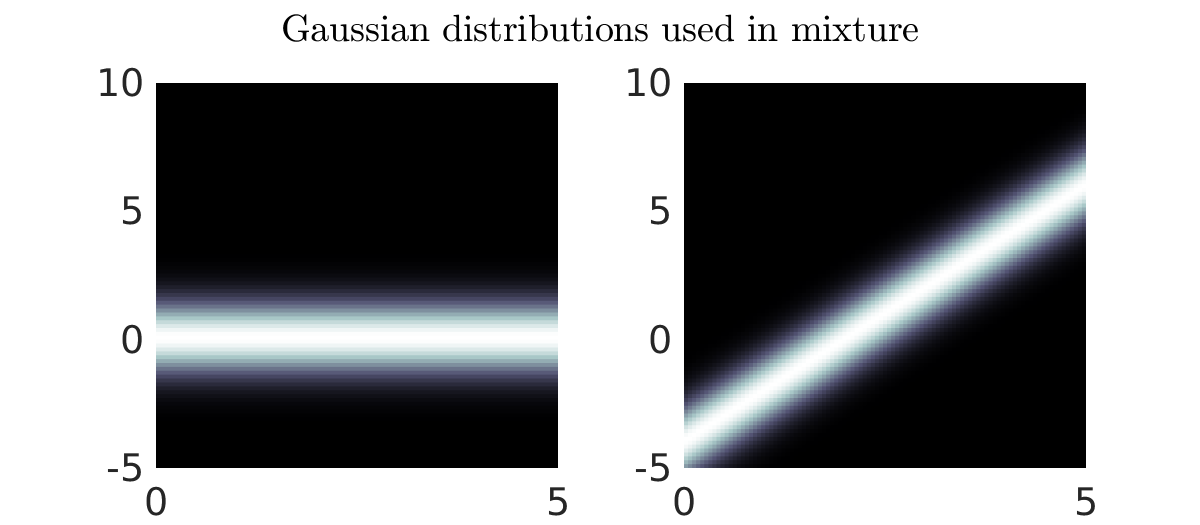
\includegraphics[width=\columnwidth]{pwagaussian.pdf}
%   \caption{Example of Gaussian Probability density functions used in mixture for identification of a 2D Piecewise Affine function with 2 modes, where \todo[verify colormap]{black represents 0 probability and white maximum }}\label{fig:pwagaussian}
% \end{figure}
\todo{Simulated annealing as in \cite{OzerovFevotte2010}}

\section{Conclusion}

A conclusion section is not required. Although a conclusion may review
the main points of the paper, do not replicate the abstract as the
conclusion. A conclusion might elaborate on the importance of the work
or suggest applications and extensions.
\begin{ack}
Simon Leglaive
\end{ack}

% \nocite{*}
\bibliography{bibliography}
% \todo[Change bibliography to the one used in the aux]{}
\end{document}
